\PassOptionsToPackage{quiet}{xeCJK}
\documentclass[declarePage]{ecnuthesis}
% 模版选项
% 模版选项是指在导入文档类的时候所指定的选项
% \documentclass[<模版选项>]{ecnuthesis}
% 可用的模版选项:
%   printMode     是否开启打印模式, 若缺省则为关闭, 反之则为开启
%   declarePage   是否生成声明页, 若缺省则不生成, 反之则生成
% 用法示例
%   \documentclass[printMode]{ecnuthesis}   (开启打印模式, 适合双面打印)
%   \documentclass{ecnuthesis}              (关闭打印模式, 适合提交电子版)

\ecnuSetup {
% 参数设置
% 允许采用两种方式设置选项:
%   1. style/... = ...
%   2. style = { ... = ... } 
% 注意事项: 
%   1. 请勿在参数设置中出现空行
%   2. "=" 两侧的空格将被忽略
%   3. "/" 两侧的空格不会被忽略
%   4. 请使用英文逗号 "," 分隔选项
%
% info 类用于输入论文信息
info = {
    title = {晶格动力学学习报告},
    % 中文标题
    %
    titleEN = {Lattice Dynamics Learning Report},
    % 英文标题
    %
    author = {刘光远},
    % 作者姓名
    %
    studentID = {10222150413},
    % 作者学号
    %
    department = {通信与电子工程学院},
    % 学院名称
    %
    major = {微电子科学与工程},
    % 专业名称
    %
    supervisor = {翁国恩},
    % 指导教师姓名
    %
    academicTitle = {副教授},
    % 指导教师职称
    %
    year  = 2022,
    % 论文完成年份
    %
    month = 11,
    % 论文完成月份
    %
    graduationYear = 22,
    % 内封面毕业届别
    % 说明:
    %   若 graduationYear 字段为空,则内封面毕业届别为 year
    %
    keywords = {晶格动力学,晶格振动,声子,声子热容,},
    % 中文关键词
    % 请使用英文逗号 "," 以分隔
    %
    keywordsEN = {x},
    % 英文关键词
    % 请使用英文逗号 "," 以分隔
    %
},
% style 类用于简单设置论文格式
style = {
    footnote  = plain,
    % 脚注编号样式
    % 可用选项:
    %   footnote = plain|circled
    % 说明:
    %   plain     脚注的编号仅为数字
    %   circled   脚注的编号为带圆圈数字 (仅限1-10)
    %   (默认选项为 plain )
    %
    numbering = arabic,
    % 章节编号样式
    % 可用选项:
    %   numbering = arabic|alpha|chinese
    % 说明:
    %   arabic    使用数字进行编号 (即理科要求)
    %   alpha     使用字母进行编号 (即外文要求)
    %   chinese   使用汉字进行编号 (即文科要求)
    %   (默认选项为 arabic )
    %
    fontCJK = fandol,
    % 中文字体选择
    % 可用选项:
    %   fontCJK = fandol|windows|mac
    % 说明:
    %   fandol    使用 TeX 自带的 fandol 字体
    %   windows   使用 Windows 系统内的字体 (中易)
    %   mac       使用 MacOS 系统内的字体
    %   (默认选项为 fandol )
    %
    fontMath = times,
    % 数学字体选择
    % 可用选项:
    %   fontMath = lm|times
    % 说明:
    %   lm        使用 TeX 自带的 Latin Modern 数学字体
    %   times     使用 Times 风格的数学字体
    %   (默认选项为 lm )
    %
    % declarePageResource = {./source/declaration.pdf},
    % 扫描版声明页 PDF 文件
    % 若该值为空则生成模版预定义的声明页;否则将插入指定路径所对应的 PDF 文件
    % 默认值为空
    %
    bibResource = {./source/thesis-ref.bib},
    % 参考文献数据源
    % 由于使用的是 biber + biblatex , 所以必须明确给出 .bib 后缀名
    %
    logoResource = {./source/inner-cover(contains_font).eps},
    % 封面插图数据源
    % 模版已自带, 位于 ./source/inner-cover(contains_font).eps
    % 默认值为空
}
}

% 需要的宏包可以自行调用
\usepackage{mwe}
\usepackage{zhlipsum}

%声明图片路径
\graphicspath{{figures/}}

\begin{document}

% 设置前置部分编号
\frontmatter

%\listoffigures
%\listoftables

% 中文摘要环境
\begin{abstract}
本篇学习报告主要记录学习晶格动力学的过程和心得。报告开头说明了晶格动力学是在波恩-奥本海默近似的基础上展开研究的
\end{abstract}

% 英文摘要环境


% 设置正文编号
\mainmatter

\chapter{问题导向} 

对于大部分固体而言,在室温附近或在比较高的温度下,它的摩尔热容都是一个固定值$3R$($R$是理想气体常数),具体值为24.6$J/mol \cdot K$。%
从能量均分学说的角度出发,在经典理论中这一规律由杜隆-珀蒂定律概括。\cite{xxx}

事实上,多数晶体在室温或高温下,热容的实验值十分吻合,如下图\ref{HC}所示。但随着温度下降,实验发现固体热容随温度同时下降。%
所以在较低的温度下,热容随温度下降而下降的现象,经典的杜隆-珀蒂定律无法解释。
\begin{figure}[htb]
    \centering
    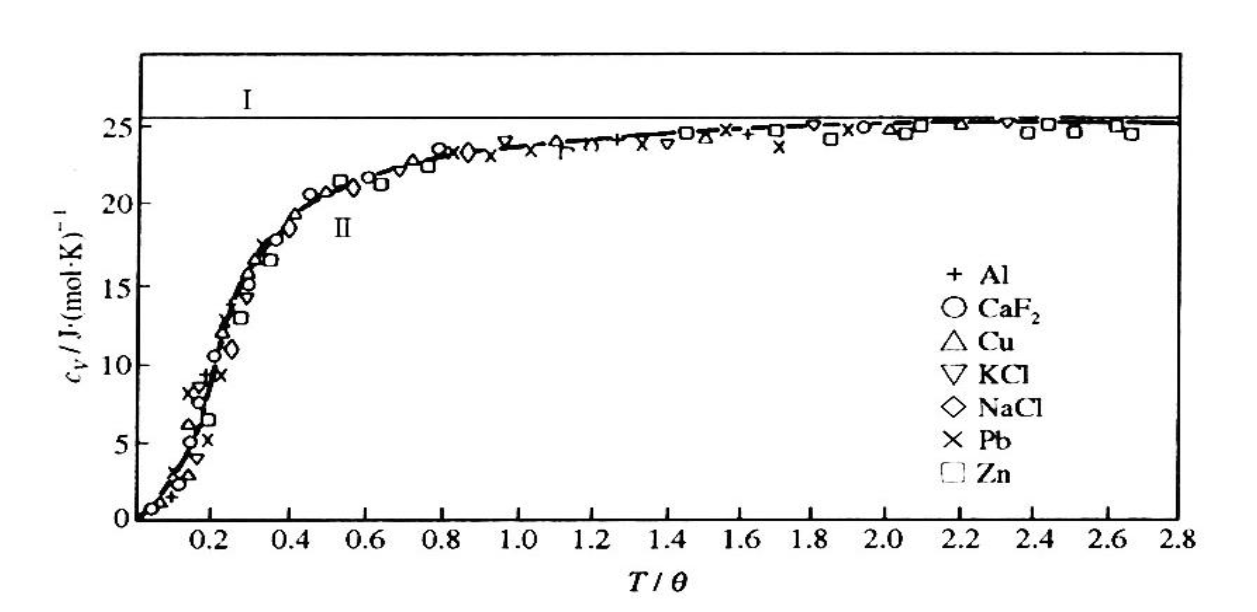
\includegraphics[width=.7\textwidth]{HC.png}
    \bicaption{固体热容实验值与理论值的比较}{Comparison Between Experiment and Theory of Heat Capacity}\label{HC}
\end{figure}

因此,围绕晶格动力学重新研究原子的运动,从而认识到原子运动对晶体的热性质(如热容)的影响,就是本次学习报告重点关注的方向。

\chapter{波恩-奥本海默近似 (Born-Oppenheimer Approximation)}

晶体表现出来的各种物理性质,背后的物理原理在于其中组成具体的基本粒子的运动规律,如原子和电子。%
以钠晶体为例,其中基本粒子的数量级在$10^{23}$,而基本粒子之间又存在着相互作用,要去考察他们各自的运动规律,%
从数学上来讲,这个多体问题是很难有严格解的。

因此,如图\ref{BOA}所示,采用波恩-奥本海默近似来简化分析,将电子运动和原子核运动分开处理。%
当我们考虑原子运动时,就不再关注电子是如何运动的;考虑电子运动的时候也同理。有关前者的研究就是本次报告的主题——晶格动力学。
\begin{figure}[htb]
    \centering
    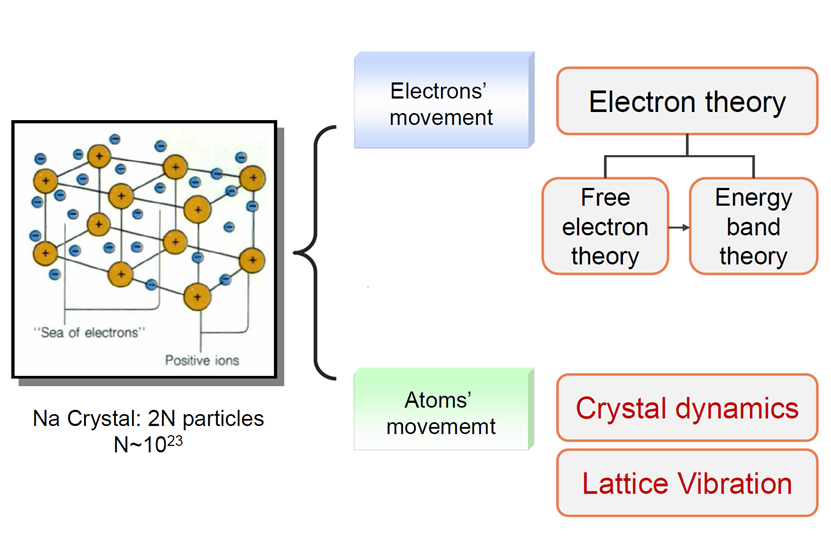
\includegraphics[width=.7\textwidth]{BOA.png}
    \bicaption{波恩-奥本海默近似}{Born-Oppenheimer Approximation}\label{BOA}
\end{figure}

\chapter{晶格振动 (Lattice Vibration)}

在晶体中,原子都是呈周期性排列,周期排列形成的点阵就是晶格,每个晶格的位置都是原子的平衡位置,所有的原子都在平衡位置做微小的振动。%
本章为研究晶格振动的基本原理,先从一维单原子链入手,分析其运动方程、边界条件、色散关系、格波形式等等,%
之后分析一维双原子相关问题并推广到三维。%
最后,对格波进行量子化分析,引入声子这个概念,从而能够方便地计算晶格振动能量。

\section{一维单原子链 (1D Monoatomic Chain)}

如图 \ref{1DMC} 所示,假设一个晶格常数为a,有N的原胞的一维单原子链,每个原胞内只有一个原子,为研究方便,先做以下两个假设:

简谐假设,原子做简谐振动,原子之间作用力为简谐力,该力满足
\begin{equation}
    F = - \beta x \text{;}
\end{equation}
最近邻假设,即原子只和最近邻原子有相互作用。
\begin{figure}[htb]
    \centering
    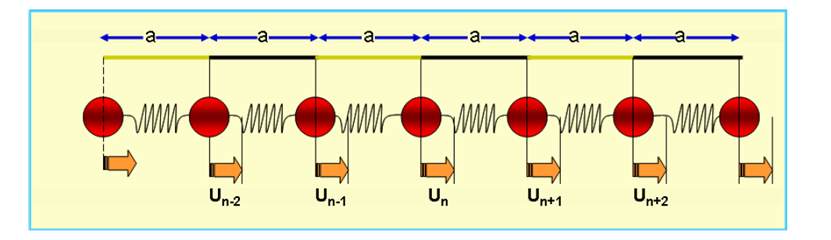
\includegraphics[width=.7\textwidth]{1DMC.png}
    \bicaption{一维单原子链}{1D Monoatomic Chain}\label{1DMC}
\end{figure}

在以上假设的基础上,对该模型进行如下分析。

\subsection{运动方程 (Equation of motion)}

对一维单原子链中第n个原子进行受力分析,即可得到它的运动方程。根据牛顿第二定律和胡克定律,有
\begin{equation}
    m \ddot{u}_n = \beta (u_{n+1} - u_n) - \beta (u_n - u_{n-1}) \text{,}
\end{equation}
化简可得
\begin{equation}
    m \ddot{u}_n = \beta (u_{n+1} - 2u_n + u_{n-1}) \text{。}
\end{equation}

式中$\beta$,可以由两个原子之间的作用势进行的泰勒展开后得到,这里不做讨论;%
$u_n$表示第n个原子的位移,$m$为原子质量。

下面对该微分方程进行求解,根据二阶微分方程解的特征,可知$u_n$应满足:
\begin{equation}
    u_n = A e^{i(kx_n - \omega t)} = A e^{i(nak - \omega t)} \text{,}
\end{equation}
将其带回原方程,可得$\omega$ \~{} $k$关系,即色散关系:
\begin{equation}
    \omega = 2 \sqrt{\frac{\beta}{m}} \left | sin \frac{ka}{2} \right | \text{,}
\end{equation}
将在3.1.3节对其进行讨论。

\subsection{波恩-卡门边界条件 (Born-Karman boundary condition)}
波恩-卡门边界条件,又称周期性边界条件。%
由于前面所考虑的运动方程实际上只适用于无穷长的链,因为所有的原子都假设有相同的运动方程,而一个有限的链两端的原子显然应当与内部的原子有所不同。%
虽然仅少数原子运动方程不同,但由于所有原子的方程都是联立的,具体解方程就复杂得多。

为了避免这种情况,采用波恩-卡门边界条件,将含N个原胞的环状链作为一个有限链的模型,如图\ref{BKBC}所示。
\begin{figure}[htb]
    \centering
    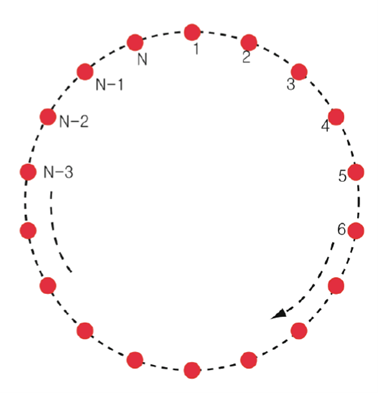
\includegraphics[width=.5\textwidth]{BKBC.png}
    \bicaption{波恩-卡门边界条件}{Born-Karman boundary condition}\label{BKBC}
\end{figure}

对于该模型,由于其周期性,显然有以下等式成立:
\begin{align}
    u_{N+1} &= u_1 \notag\\
    u_{N+n} &= u_n \text{。}
\end{align}

将该式带入运动方程,可以得到关于k的一系列取值:
\begin{equation}
    k = \frac{2\pi}{Na}m \text{,}
\end{equation}
其中,m可以取所有整数。

由此可知,k的取值并不是连续的,而是一个个分立的值。%
但是由于在晶体中,N是一个及其大的数,因此,相较于布里渊区的大小,k可以当作是准连续的一个量。%
此处得到的k的取值,将在后面分析格波数量时起到关键作用。

\subsection{色散关系 (Dispersion relation)}

% 正文后部分
\backmatter
% 导入参考文献 (需要通过 latexmk 编译后才能显示)
\PrintReference

\end{document}